% This is samplepaper.tex, a sample chapter demonstrating the
% LLNCS macro package for Springer Computer Science proceedings;
% Version 2.21 of 2022/01/12
%
\documentclass[runningheads]{llncs}
%
\usepackage[T1]{fontenc}
% T1 fonts will be used to generate the final print and online PDFs,
% so please use T1 fonts in your manuscript whenever possible.
% Other font encondings may result in incorrect characters.
%
\usepackage{graphicx}
% Used for displaying a sample figure. If possible, figure files should
% be included in EPS format.
%
% If you use the hyperref package, please uncomment the following two lines
% to display URLs in blue roman font according to Springer's eBook style:
%\usepackage{color}
%\renewcommand\UrlFont{\color{blue}\rmfamily}
%\urlstyle{rm}
%
\usepackage{amsmath}
\usepackage{bbm}
\usepackage{bm}
\usepackage{siunitx}
\usepackage{tikz}
 \usepackage{amssymb}
\usetikzlibrary{arrows.meta,calc,angles,quotes,positioning}
\usepackage{subcaption}
\usepackage{pdflscape}
\usepackage{hyperref}
% \usepackage{color}
% \usepackage{listings}
%     \lstdefinelanguage{Matlab}{
%       keywords={break,case,catch,continue,else,elseif,end,for,function,
%         global,if,otherwise,persistent,return,switch,try,while},
%       keywordstyle=\color{blue}\bfseries,
%       commentstyle=\color{gray}\ttfamily,
%       stringstyle=\color{red},
%     }
    
%     \lstdefinestyle{matlab}{
%       language=Matlab,
%       basicstyle=\ttfamily\small,
%       numbers=left,
%       numberstyle=\tiny\color{gray},
%       stepnumber=1,
%       numbersep=6pt,
%       showstringspaces=false,
%       breaklines=true,
%       frame=single,
%       tabsize=2,
%       captionpos=b
%     }
%     % \lstset{style=matlab}
\usepackage{listings}
\usepackage{xcolor}
\definecolor{mygreen}{RGB}{28,172,0} % color values Red, Green, Blue
\definecolor{mylilac}{RGB}{170,55,241}
\lstset{
  language=Matlab,
  basicstyle=\ttfamily\small,
  keywordstyle=\color{blue}\bfseries,
  commentstyle=\color{mygreen}\ttfamily,
  stringstyle=\color{mylilac},
  numbers=left,
  numberstyle=\tiny\color{gray},
  numbersep=6pt,
  showstringspaces=false,
  breaklines=true,
  frame=single,
  tabsize=2,
  captionpos=b
}

\newcommand{\vehicle}{\textsc{Vehicle}}
\newcommand{\marabou}{\textsc{Marabou}}


\begin{document}
%
\title{Safety Evaluation of Neural Network Control for Drone Delivery Systems}
%
%\titlerunning{Abbreviated paper title}
% If the paper title is too long for the running head, you can set
% an abbreviated paper title here
%

%ORCID IDs if we want to include them later
% Calum \orcidID{0009-0004-1234-2494}
% Julia \orcidID{}
% Ruchira \orcidID{}

\author{
Calum Arnott\thanks{Equal contribution}\inst{1,2}
\and
Julia López Gómez\protect\footnotemark[1]\inst{1,2}
\and
Ruchira Ray\protect\footnotemark[1]\inst{1,2}
}

%
\authorrunning{C. Arnott et al.}
% First names are abbreviated in the running head.
% If there are more than two authors, 'et al.' is used.
%
\institute{
University of Edinburgh, UK \\ \email{\{C.R.Arnott,J.Lopez-Gomez,R.Ray-3\}@sms.ed.ac.uk} 
\and 
Heriot-Watt University, UK \\ \email{\{cra4000,jl4065,rr4033\}@hw.ac.uk}
}
%
\maketitle              % typeset the header of the contribution
%

\begin{abstract}
% The abstract should briefly summarize the contents of the paper in
% 150--250 words.
Neural network controllers are increasingly used in safety-critical cyber-physical systems due to their ability to approximate complex non-linear control policies. However, providing guarantees about their behaviour remains challenging, particularly when such controllers are deployed in closed loop with non-linear dynamics. This paper presents a case study on the robustness and verification of a neural network controller for a quadrotor drone performing winch-based payload delivery with a tethered load. An expert PID controller is first designed to stabilise the coupled drone-payload system in desired setpoints and is used to generate training data. A NN controller is then trained to approximate the expert policy, and adversarial training and property-driven training are incorporated to improve robustness and bias the controller toward safe behaviour and property compliance. The learned controllers are evaluated using three complementary verification techniques. First, controller-level formal property verification is performed using the \vehicle\ specification language and the \marabou\ solver to assess properties such as bounded actuation or correct control direction. Second, finite-time reachability analysis of the closed-loop system is conducted using CORA, revealing scalability limitations due to non-linear dynamics and dimensionality. Third, empirical robustness is evaluated under adversarial input perturbations, complemented by explainability analysis using LIME and Integrated Gradients to assess feature sensitivity and stability. This case study highlights the interaction between training strategies and verifiability, and showcases current challenges in verifying NN controllers for aerial robotics applications.
\end{abstract}



\keywords{Neural Network Control \and Uncrewed Aerial Vehicle \and Verification of Cyber-Physical Systems \and Machine Learning.}

% \subsection*{Author Contributions}

% \paragraph{Calum Arnott}
% developed the continuous-time dynamics model of the tethered drone–payload system, including the underlying physical assumptions and equations of motion. He designed and implemented the baseline PID controller and simulator used for closed-loop control and data generation. Calum also specified and evaluated selected verification properties, and carried out all reachability analysis using CORA, including both open-loop and closed-loop reachability experiments and associated analysis of set explosion and numerical limitations.

% \paragraph{Julia López Gómez}
% designed and implemented the full neural network control pipeline, including dataset generation, network architecture design, training, validation, and closed-loop integration with the system dynamics and simulations. She specified and implemented the verification properties in Vehicle, including robustness properties such as Lipschitz. Julia developed learning objectives to integrate these properties into NN verification through property-driven training. 

% \paragraph{Ruchira Ray}
% implemented adversarial attacks and adversarial training methods for the neural network controller, including PGD-based perturbations used to model sensor noise and external disturbances. She conducted robustness experiments under adversarial perturbations and contributed to the analysis of robustness improvements resulting from adversarial training, as well as the associated evaluation plots and comparisons.


% \subsection*{Author Contributions}

% \paragraph{Calum Arnott}
% System dynamics; PID controller design; simulator implementation; data generation support; controller-level property specification; open- and closed-loop reachability analysis using CORA; analysis of set explosion and numerical limitations.

% \paragraph{Julia López Gómez}
% Neural network control pipeline design and implementation; dataset generation; closed-loop integration with simulations; controller-level property specification in Vehicle; robustness and Lipschitz-related properties; property-driven training loss formulation and integration.

% \paragraph{Ruchira Ray}
% PGD/FGSM attack and adversarial training implementation for robustness; LIME explainability; Integrated Gradients explainability; empirical robustness evaluation under bounded perturbations and result visualisation.


%
%
%
\section{Introduction}
\label{sec:introduction}

% \subsection{Contributions}
We introduce a novel verification case study for an aerial delivery cyber-physical system: a planar quadrotor with an underslung payload connected via a tether. The benchmark preserves key non-linear couplings between vehicle motion, payload swing, and tether dynamics while remaining sufficiently structured to integrate with current neural network verification tools. Using this benchmark, we develop an expert PID controller and train a neural network controller by behavioural cloning, providing a learned control policy suitable for both empirical evaluation and formal analysis.

To improve robustness and encourage safe behaviour, we investigate robustness-based training, including adversarial training under bounded input perturbations, and property-driven training (PDT), in which controller-level specifications are translated into differentiable penalty terms and integrated into the learning objective. We analyse how these training strategies affect both empirical robustness and verifiability. To support interpretability and diagnostic insight, we apply explainability analysis using LIME \cite{ribeiro_why_2016} and Integrated Gradients~\cite{sundararajan2017axiomatic} to compare feature importance and stability between baseline and robustly trained controllers.

Finally, we evaluate the learned controllers using three complementary assurance techniques at different levels of abstraction: (i) controller-level formal property verification of the neural network in isolation using the \vehicle\ specification language \cite{vehicle} with the \marabou\ solver \cite{wu2024marabou}; (ii) system-level finite-horizon closed-loop reachability analysis using CORA \cite{cora}; and (iii) empirical robustness evaluation via adversarial perturbation testing. All code for simulation, training, and verification is released as open source\footnote{\url{https://github.com/calumarnott/f21zk.git}}.


\subsection{Drone Delivery}
The use of Uncrewed Aerial Vehicles (UAVs)--more commonly known as drones--for the delivery of packages has become increasingly widespread in both rural and urban environments. Drone delivery has been used to improve access to healthcare and ensure time-critical delivery of medical goods, such as vaccines \cite{haidari_economic_2016,enayati_vaccine_2023,ospina-fadul_cost-effectiveness_2025} and blood \cite{nisingizwe_effect_2022,ling_aerial_2019,glauser_blood-delivering_2018,amukele_can_2015}. In urban environments, drones are increasingly being developed for last-mile delivery of food and consumer goods \cite{brunner_urban_2019,mazur_commercial_2025}. Operation of drones, particularly in urban environments, requires adherence to strict safety and reliability requirements administered by local flight aviation authorities.

Several mechanisms have been utilised for delivering packages using drones, including parachute-based delivery \cite{glauser_blood-delivering_2018,ho_optimizing_2025,hughes_autonomous_2023} and servo-actuated mechanisms \cite{maheshwar_development_2024,iqbal_servo_2016}. Whilst these approaches offer a straightforward method for dropping the payload (‘package’), neither offers precise control over the payload descent dynamics. Increasingly, winch based mechanisms are explored in which the payload is suspended beneath the drone on a tether and lowered to the ground using a motorised winch \cite{poulsen_uncrewed_2024,crowe_design_2025,pillai_optimizing_2025}. This configuration has several practical advantages, including the ability to deliver a payload without requiring a human to approach the drone itself, thereby reducing the risk of collision with hazardous rotating components such as propellers. Nevertheless, winched delivery introduces safety concerns to address, including payload swing, slack or excessive tension in the tether, winch overload, and collisions with the surrounding environment. 

The resulting drone-payload system shows coupled multi-body dynamics along with non-linear effects. Ensuring safe operation therefore requires careful control design and rigorous analysis.

\subsection{Neural Network Control of Cyber-Physical Systems}
Neural Networks (NNs) have been utilised for control in cyber-physical systems \cite{musa_deep_2023}, including for UAV applications \cite{amer_deep_2021,yu_quadrotor_2023}. NNs are appealing due to their ability to learn complex non-linear control mappings, to cope with uncertainty, and to perform well when accurate modelling of system dynamics is difficult \cite{gu_uav_2020}. These properties are particularly relevant in aerial robotics, where system dynamics include coupled translational and rotational motion, non-linear actuator behaviour, and environmental disturbances such as wind. However, the adoption of NN controllers in safety-critical applications remains limited by the lack of formal guarantees on their behaviour. Verification of NNs as controllers is a burgeoning research field \cite{sun_formal_2019,seshia_formal_2018,genin_formal_2022}, and formal verification techniques are desirable for assuring safety in systems that operate in close proximity to people and the environment, such as delivery drones.

From a verification perspective, the drone delivery system with an underslung payload presented has several distinguishing challenges from existing cyber-physical system (CPS) benchmarks. Firstly, the NN controller is based on a regression network, which produces continuous-valued control outputs rather than discrete actions or class labels. Moreover, the closed-loop dynamics of the combined drone–payload system are non-linear and relatively high-dimensional, making reachability analysis computationally challenging. Additionally, safety is not naturally expressed as simple avoidance of unsafe regions in the state space; rather, desired behaviour is more naturally characterised as maintaining bounded deviation from a target trajectory or operating regime. Though prior benchmarks have addressed the verification of neural network controllers for a quadcopter drone \cite{lopez_arch-comp23_2023}, the inclusion of an underslung payload increases the complexity of the system as the controller must simultaneously regulate the motion of the drone and the payload, which are highly coupled dynamically. 

This places the drone-payload system at the boundary of what existing neural network verification and reachability tools can handle in practice.

% \subsection{Contributions}

% This paper presents a case study on neural network verification for an aerial delivery system, consisting of a quadrotor UAV (drone) with a tethered payload. Focus is placed on evaluating existing verification tools and methodologies when applied to a novel CPS. To this end, we develop a NN controller for the drone-payload system using behaviour cloning from an expert Proportional-Integral-Derivative (PID) controller. We derive a planar model of the combined drone–payload dynamics, making explicit assumptions and simplifications that preserve the key non-linear couplings while simplifying the system sufficiently for analysis with the verification tools assessed.

% Robustness of the NN controller is investigated by analysing its sensitivity to bounded input perturbations and by applying adversarial training techniques. We apply explainable AI techniques like LIME \cite{ribeiro_why_2016} to analyse feature importance in the controller’s decision-making process and to compare baseline and adversarially trained networks. Based on our results, we identify where verification succeeds, where it fails, and what these outcomes imply for the verification of NN controllers in safety-critical aerial robotics. The insights gained from this case study highlight gaps between realistic CPS requirements and current verification tooling, and point towards directions for future benchmark design and tool development.

% We formalise a set of physically meaningful, controller-level safety properties, such as bounded actuation and correct control direction, which are interpretable from an engineering perspective. These properties are evaluated at the neural network level using Vehicle with the Marabou solver. In addition, we perform finite-time closed-loop reachability analysis of the NN-controlled system using CORA, highlighting the effects of nonlinear dynamics, dimensionality, and set explosion on verification scalability.

% All code developed for this case study, including the drone-payload simulation environment, neural network training scripts, and verification analyses, is made publicly available in our GitHub repository\footnote{\url{https://github.com/calumarnott/f21zk.git}}.




% This paper presents a case study on neural network verification for an aerial delivery system, consisting of a quadrotor UAV (drone) with a tethered payload. Focus is placed on evaluating existing verification tools and methodologies when applied to a novel CPS. To this end, we develop a NN controller for the drone-payload system using behaviour cloning from an expert Proportional-Integral-Derivative (PID) controller. We derive a planar model of the combined drone–payload dynamics, making explicit assumptions and simplifications that preserve the key non-linear couplings while simplifying the system sufficiently for analysis with the verification tools assessed.

% Robustness of the NN controller is investigated by analysing its sensitivity to bounded input perturbations and by applying adversarial training techniques. We apply explainable AI techniques like LIME \cite{ribeiro_why_2016} to analyse feature importance in the controller’s decision-making process and to compare baseline and adversarially trained networks. We also formalise a set of physically meaningful, controller-level safety properties, such as bounded actuation and correct control direction, which are interpretable from an engineering perspective. These properties are evaluated at the neural network level using Vehicle with the Marabou solver. In addition, we perform finite-time closed-loop reachability analysis of the NN-controlled system using CORA, highlighting the effects of nonlinear dynamics, dimensionality, and set explosion on verification scalability.

% All code developed for this case study, including the drone-payload simulation environment, neural network training scripts, and verification analyses, is made publicly available in our GitHub repository\footnote{\url{https://github.com/calumarnott/f21zk.git}}.




% Firstly, we verify properties of the neural network controller in isolation, independent of the system dynamics. This class of analysis focuses on infinite time-horizon properties of the controller itself, such as bounded control outputs and robustness to bounded input perturbations. We perform controller-level verification using the Marabou SMT-based neural network verifier, accessed through the Vehicle specification language. Vehicle provides a higher-level interface for expressing verification properties in physically meaningful units, thereby helping bridge the embedding gap between the physical domain and the vectorised representations required by neural network verifiers.

% Secondly, we analyse the closed-loop behaviour of the neural network controller together with the non-linear system dynamics using finite time-horizon reachability analysis. .This class of verification determines whether all trajectories originating from a specified initial set avoid unsafe regions over a bounded time interval. For this we use CORA , a framework implemented in MATLAB, which supports non-linear continuous-time dynamics and neural network controllers. This enables system-level safety analysis that cannot be addressed by controller-level verification alone.

% Finally, we incorporate robustness-oriented training techniques from the machine learning literature to improve both empirical performance and verifiability. In particular, we apply projected gradient descent (PGD)–based adversarial training to the neural network controller and compare a baseline model against an adversarially trained variant. The two controllers are evaluated with respect to performance under adversarial perturbations as well as their ability to satisfy formal verification properties. In addition, we explore property-driven training approaches that directly optimise the neural network to satisfy standard robustness specifications, enabling a direct comparison of verification outcomes before and after robustness-oriented training.



% \section{Background}
% \label{sec:background}
% \subsection{Neural Network Control}
We adopt a standard closed-loop negative feedback controller as in \cite{kessler_neural_2025}. At each control step, the controller receives information about the current state, and computes actuator commands that act to control the system through its dynamics. In this regard, the controller can be seen as a mapping from system states to control inputs, which determines the closed-loop behaviour over time. 

While controllers typically use control laws derived from theory, using analytical models of the dynamics, neural network controllers offer an alternative for when accurate system modelling is challenging, when data-driven methods are preferable, or when adaptation to new operating conditions is required. 

\subsection{Verification Tools}

This case study relies on three complementary classes of neural network verification and robustness techniques.

Firstly, we verify properties of the neural network controller in isolation, independent of the system dynamics. This class of analysis focuses on infinite time-horizon properties of the controller itself, such as bounded control outputs and robustness to bounded input perturbations. We perform controller-level verification using the \marabou\ SMT-based neural network verifier, accessed through the \vehicle\ specification language. \vehicle\ provides a higher-level interface for expressing verification properties in physically meaningful units, thereby helping bridge the embedding gap between the physical domain and the vectorised representations required by neural network verifiers.

Secondly, we analyse the closed-loop behaviour of the neural network controller together with the non-linear system dynamics using finite time-horizon reachability analysis. .This class of verification determines whether all trajectories originating from a specified initial set avoid unsafe regions over a bounded time interval. For this we use CORA , a framework implemented in MATLAB, which supports non-linear continuous-time dynamics and neural network controllers. This enables system-level safety analysis that cannot be addressed by controller-level verification alone.

Finally, we incorporate robustness-oriented training techniques from the machine learning literature to improve both empirical performance and verifiability. In particular, we apply projected gradient descent (PGD)–based adversarial training to the neural network controller and compare a baseline model against an adversarially trained variant. The two controllers are evaluated with respect to performance under adversarial perturbations as well as their ability to satisfy formal verification properties. In addition, we explore property-driven training approaches that directly optimise the neural network to satisfy standard robustness specifications, enabling a direct comparison of verification outcomes before and after robustness-oriented training.




\section{Modelling}
\label{sec:modelling}
We model a quadcopter drone transporting a payload via a tethered winch mechanism. To improve tractability for verification, the dynamics are simplified with the following assumptions: planar motion in the $x$--$z$ plane; a rigid, symmetric quadcopter with mass concentrated at its centre of mass; a massless, inextensible tether that remains taut; pure axial thrust from the rotors; and no aerodynamic drag or external disturbances. The tether tension is resolved via a quasi-static iteration at each timestep, assumed accurate for sufficiently small integration steps. These assumptions preserve the dominant non-linear couplings between the drone and payload while yielding a model suitable for formal analysis.

\subsection{State, Controls, and Parameters}

The system state captures the planar motion of the quadcopter and the dynamics of the tethered payload:
\[
\bm{s} =
\begin{bmatrix}
x_q & z_q & \theta & \dot{x}_q & \dot{z}_q & \dot{\theta} & \ell & \phi & \dot{\ell} & \dot{\phi}
\end{bmatrix}^{\!\top}.
\]

The control input consists of the individual rotor thrusts and the commanded tether feed rate:
\[
\bm{u} =
\begin{bmatrix}
T_1 & T_2 & T_3 & T_4 & u_\ell
\end{bmatrix}^{\!\top}.
\]

Here, $x_q$ and $z_q$ denote the quadcopter centre-of-mass position, $\theta$ is the pitch angle, $\ell$ is the tether length, and $\phi$ is the payload swing angle measured from the vertical. Dots denote time derivatives.

The system's physical parameters are the quadcopter mass $m_q$, payload mass $m_p$, pitch-axis inertia $I_q$, gravitational acceleration $g$, and rotor arm length $d$.

\subsection{Equations of Motion}

The translational dynamics of the quadcopter are given by
\begin{equation}
m_q
\begin{bmatrix}
\ddot{x}_q \\[2pt] \ddot{z}_q
\end{bmatrix}
=
\bm{F}_{\text{thrust}}
+ Q\,\bm{u}(\phi)
- m_q g
\begin{bmatrix}
0 \\ 1
\end{bmatrix},
\end{equation}
where $\bm{F}_{\text{thrust}}$ is the total thrust force and $Q$ is the tether tension.

The rotational dynamics about the pitch axis are
\begin{equation}
I_q\,\ddot{\theta} = \tau,
\end{equation}
with $\tau$ denoting the applied pitch torque.

The payload dynamics satisfy
\begin{equation}
m_p\,\ddot{\bm{p}}_p =
- m_p g
\begin{bmatrix}
0 \\ 1
\end{bmatrix}
- Q\,\bm{u}(\phi),
\end{equation}
where $\bm{p}_p$ is the payload position.

Projecting the payload dynamics onto the tether frame yields the swing equation
\begin{equation}
\ell\,\ddot{\phi} + 2\,\dot{\ell}\,\dot{\phi}
=
- g\,\sin\phi
+
\begin{bmatrix}
\ddot{x}_q \\[2pt] \ddot{z}_q
\end{bmatrix}
\!\cdot \bm{t}(\phi),
\end{equation}
and the radial equation
\begin{equation}
m_p(\ddot{\ell} - \ell \dot{\phi}^2)
=
m_p g \cos\phi
- Q
+
m_p
\begin{bmatrix}
\ddot{x}_q \\[2pt] \ddot{z}_q
\end{bmatrix}
\!\cdot \bm{u}(\phi).
\end{equation}

Solving for the tether tension gives
\begin{equation}
Q =
m_p\!\left[
g \cos\phi
+
\begin{bmatrix}
\ddot{x}_q \\[2pt] \ddot{z}_q
\end{bmatrix}
\!\cdot \bm{u}(\phi)
- (\ddot{\ell} - \ell \dot{\phi}^2)
\right].
\end{equation}

The tether feed rate is controlled directly by the winch input,
\begin{equation}
\dot{\ell} = u_\ell.
\end{equation}

All geometric definitions and intermediate derivations are provided in Appendix~\ref{ap:tether_derivation}.

% ---------------------

% % \subsection{Summary and Assumptions}

% We derive the dynamics of our system comprising a quadcopter drone and a tethered payload. To improve tractability of the verification task, we simplify the dynamics formulation by considering planar (2D) motion; a rigid, symmetric drone with mass concentrated at its centre of mass; a massless, inextensible tether between the drone and payload; pure axial thrust rotors; and no aerodynamic drag or external disturbances. 

% % \begin{enumerate}
% %     \item \textit{Planar motion:} Both drone and payload move only in the $x$--$z$ plane; there is no yaw or roll motion.
% %     \item \textit{Rigid symmetric quadcopter:} The drone is a single rigid body with its mass concentrated at its centre of mass.
% %     \item \textit{Massless, inextensible tether:} Always taut ($Q>0$) with no elasticity or mass. Tether length $\ell$ varies only via the commanded feed rate $u_\ell$.
% %     \item \textit{Axial thrust:} Each rotor produces thrust only along its body axis (no drag or gyroscopic coupling). Thrust changes instantaneously.
% %     \item \textit{No aerodynamic drag:} Air resistance on the quadcopter and payload is neglected.
% %     \item \textit{No external disturbances:} Wind and other perturbations are ignored.
% %     \item \textit{Quasi-static tether iteration:} The tether tension $Q$ depends on the drone acceleration terms, which itself depends on $Q$. 
% %     Instead of solving implicitly, we iterate once or twice per timestep, which is assumed accurate for small timesteps (e.g., $dt < 0.05~\mathrm{s}$.)
% % \end{enumerate}

% \subsection{State and Controls}
% The system state captures the planar motion of the quadcopter and the dynamics of the tethered payload. Specifically, it includes the lateral and vertical position of the quadcopter’s centre of mass, its pitch angle, and the corresponding time derivatives. In addition, the state incorporates the tether length, the payload swing angle relative to the vertical, and the rates of change of these quantities. The control input consists of the individual thrust forces applied by the four rotors and the commanded tether feed rate.
% \[
% \bm{s} =
% \begin{bmatrix}
% x_q & z_q & \theta & \dot{x}_q & \dot{z}_q & \dot{\theta} & \ell & \phi & \dot{\ell} & \dot{\phi}
% \end{bmatrix}^{\!\top},
% \quad
% \bm{u} =
% \begin{bmatrix}
% T_1 & T_2 & T_3 & T_4 & u_\ell
% \end{bmatrix}^{\!\top}
% \]

% where \(x_q, z_q\) are the quadcopter centre of mass (COM) coordinates, \(\theta\) is the pitch angle, 
% \(\ell\) is the rope length, and \(\phi\) is the rope swing angle from vertical.
% Dots denote time derivatives.

% % \subsection{Parameters}
% The parameters of the system are the mass of the quadcopter and payload, \(m_q, m_p\), the pitch-axis inertia, \(I_q\), gravitational acceleration, \(g\), and the rotor arm length  (distance from COM to rotor thrust line), \(d\).

% \subsection{Tether Geometry and Kinematics}

% We consider planar motion of a quadcopter with a payload suspended beneath it by a massless, inextensible tether of variable length $\ell$. The configuration of the tether is parameterised by the swing angle $\phi$, measured from the vertical. To describe the payload motion conveniently, we define unit vectors aligned with and perpendicular to the tether as
% \[
% \bm{u}(\phi) =
% \begin{bmatrix}
% \sin\phi \\[2pt] -\cos\phi
% \end{bmatrix},
% \qquad
% \bm{t}(\phi) =
% \begin{bmatrix}
% \cos\phi \\[2pt] \sin\phi
% \end{bmatrix},
% \]
% where $\bm{u}$ points from the quadcopter toward the payload and $\bm{t}$ is tangential to the payload swing, orthogonal to $\bm{u}$.

% The payload position $\bm{p}_p$ is expressed relative to the quadcopter centre of mass $(x_q,z_q)$ as

% \begin{equation}
%     \bm{p}_p =
%     \begin{bmatrix}
%     x_q \\ z_q
%     \end{bmatrix}
%     + \ell\,\bm{u}(\phi).  
% \end{equation}


% Differentiating twice yields the payload acceleration
% \begin{equation}
%     \ddot{\bm{p}}_p =
%     \begin{bmatrix}
%     \ddot{x}_q \\[2pt] \ddot{z}_q
%     \end{bmatrix}
%     + (\ddot{\ell} - \ell \dot{\phi}^{2})\, \bm{u}
%     + (2\dot{\ell}\dot{\phi} + \ell \ddot{\phi})\, \bm{t},
% \end{equation}

% which explicitly captures the coupling between quadcopter motion, tether length variation, and payload swing.

% \subsection{Forces and Equations of Motion}

% The drone is subject to the total thrust force $\bm{F}_{\text{thrust}}$, gravitational force $m_q g$, and the tether tension $Q\,\bm{u}$. The payload experiences gravitational force and an equal and opposite tether force, consistent with Newton’s third law. A free-body diagram is shown in Appendix~\ref{ap:fbd}.

% Applying Newton’s second law, the translational dynamics of the quadcopter are given by

% \begin{equation}
%     m_q
%     \begin{bmatrix}
%     \ddot{x}_q \\[2pt] \ddot{z}_q
%     \end{bmatrix}
%     =
%     \bm{F}_{\text{thrust}}
%     + Q\,\bm{u}
%     - m_q g
%     \begin{bmatrix}
%     0 \\ 1
%     \end{bmatrix},
% \end{equation}

% where the sign convention of the tether force is embedded in the definition of $\bm{u}$. The rotational dynamics about the pitch axis are

% \begin{equation}
%     I_q\,\ddot{\theta} = \tau,
% \end{equation}

% with $I_q$ the quadcopter pitch inertia and $\tau$ the applied torque.

% The translational dynamics of the payload follow as

% \begin{equation}
%     m_p\,\ddot{\bm{p}}_p =
%     - m_p g
%     \begin{bmatrix}
%     0 \\ 1
%     \end{bmatrix}
%     - Q\,\bm{u}.
% \label{eq:payload_dyn}
% \end{equation}

% % \subsection{Payload Dynamics in Tether Coordinates}
% \subsection{Payload Dynamics in Tether Coordinates and Winch Model}

% To obtain equations governing the swing and tension dynamics, Eq.~\ref{eq:payload_dyn} is projected onto the tangential and radial directions defined by $\bm{t}(\phi)$ and $\bm{u}(\phi)$.

% Projection onto the tangential direction yields the swing equation

% \begin{equation}
%     \ell\,\ddot{\phi} + 2\,\dot{\ell}\,\dot{\phi}
%     =
%     - g\,\sin\phi
%     +
%     \begin{bmatrix}
%     \ddot{x}_q \\[2pt] \ddot{z}_q
%     \end{bmatrix}
%     \!\cdot\bm{t}(\phi),
% \end{equation}

% which shows how payload oscillations are driven both by gravity and by quadcopter accelerations.

% Projection onto the radial direction gives
% \begin{equation}
%     m_p(\ddot{\ell} - \ell \dot{\phi}^2)
%     =
%     m_p g \cos\phi
%     - Q
%     +
%     m_p
%     \begin{bmatrix}
%     \ddot{x}_q \\[2pt] \ddot{z}_q
%     \end{bmatrix}
%     \!\cdot\bm{u}(\phi),
% \end{equation}

% from which the tether tension can be expressed as
% \begin{equation}
%     Q =
%     m_p\!\left[
%     g \cos\phi
%     +
%     \begin{bmatrix}
%     \ddot{x}_q \\[2pt] \ddot{z}_q
%     \end{bmatrix}
%     \!\cdot\bm{u}(\phi)
%     - (\ddot{\ell} - \ell \dot{\phi}^2)
%     \right].      
% \end{equation}

% % \subsection{Winch Model}

% The tether length $\ell$ is controlled via a motorised winch. Two models are considered. In the simplest case, the tether feed rate is assumed to track the control input directly: $\dot{\ell} = u_\ell$.
% % \begin{equation}
% %     \dot{\ell} = u_\ell.   
% % \end{equation}


\section{Implementation}
\label{sec:implementation}
This section describes the expert controller and simulation framework used to generate training data, followed by the learning pipeline used to train a regression neural network controller via behavioural cloning.

\subsection{Expert PID Controller}

Each controlled variable $x_i$ is governed by a PID law of the form
\begin{equation}
u_i(t) = K_{p,i} e_i(t) + K_{i,i} \int_0^t e_i(\tau)\,d\tau + K_{d,i} \frac{d e_i(t)}{dt},
\end{equation}
where $e_i(t) = x_{i,\text{ref}}(t) - x_i(t)$ denotes the tracking error.

Independent PID controllers are implemented for the following objectives:
\begin{align*}
u_x &: \text{horizontal quadcopter position } (x_q), \\
u_z &: \text{vertical quadcopter position } (z_q), \\
u_\phi &: \text{payload swing damping } (\phi \rightarrow 0), \\
u_\theta &: \text{quadcopter pitch stabilisation } (\theta), \\
u_\ell &: \text{tether feed control } (\ell_{\text{ref}}(t)).
\end{align*}

A cascaded control structure is used, with outer-loop controllers regulating position and payload motion, and inner-loop controllers stabilising vehicle attitude and velocity. Additional details of the implementation are included in Appendix~\ref{ap:pid}. For simplicity, and to reduce the dimensionality of the learning problem, the neural network controller is trained assuming a fixed tether length; consequently, the tether feed controller is inactive during data generation.

The PID controller is not intended to be optimal, but rather to provide a reliable and interpretable expert suitable for supervised learning. As a result, the behaviour and safety properties of the learned neural network controller are inherently constrained by the coverage and quality of the expert demonstrations.

\subsection{Dataset Generation}

The expert PID-controlled simulation is used to generate training data for the NN controller. Trajectories are generated by sampling a range of initial conditions to reach a reference setpoint, and logging the resulting state, error, and control tuples at each simulation step. The data generation pipeline is outlined in Fig.~\ref{fig:data_gen}. At each time step $t$, the input to the learning model --the dataset features-- consists of the system state $\bm{s}_t$ together with a vector of tracking errors $\bm{e}_t$, defined with respect to the desired reference trajectory or setpoint:
\[
\bm{e}_t = \bm{s}_{\text{ref}}(t) - \bm{s}_t.
\]

The resulting dataset is given by
\[
\mathcal{D} = \{ (\bm{s}_t, \bm{e}_t), \bm{u}_t \}_{t=0}^{T},
\]
where $\bm{u} = \pi_{\text{PID}}(\bm{s})$ denotes the control action generated by the PID controller.

\begin{figure}[t]
    \centering
    \includegraphics[width=0.82\linewidth]{figs/data-generation-pipeline.pdf}
    \caption{Dataset generation pipeline using expert PID controller in simulation. The numerical simulation framework used with the expert PID controller to update the system dynamics is detailed in Appendix~\ref{ap:num_sim_framework}.}
    \label{fig:data_gen}
\end{figure}



% This formulation defines a supervised regression problem in which the neural network is trained to approximate the expert policy mapping from states and tracking errors to continuous-valued control outputs.







% \subsection{Neural Network Controller}
% \subsubsection{Architecture}
% The controller is implemented as a feed-forward neural network that maps the system state $\bm{s}$ to continuous-valued control outputs $\bm{u}$. The network architecture is designed to support regression-based control and real-time inference, while remaining compatible with existing neural network verification tools.

% include number of layers, hidden dimensions, activation functions, and output normalisation etc

% \subsubsection{Training}

% Training is performed using supervised learning on the dataset generated by the expert controller. The neural network parameters are optimised to minimise a regression loss between the predicted control outputs and the expert commands.

% The training procedure, including dataset splitting, loss functions, optimisation algorithms, and hyperparameter choices, is described in detail in the following section.

% \subsubsection{Adversarial Training for Robustness}

% To improve robustness of the learned controller to bounded perturbations in the input state, adversarial training is applied during neural network training. Perturbations are introduced at the input level to simulate sensor noise and modelling uncertainty, encouraging the network to learn a smoother and more stable control policy.

\subsection{Neural Network Controller}

The learned controller is implemented as a feed-forward neural network that approximates the expert PID policy via supervised behavioural cloning. The network maps the current system state and tracking errors to continuous-valued control outputs, and is evaluated in closed loop using the nonlinear system dynamics described in Section~\ref{sec:modelling}.

\subsubsection{Architecture}

The controller is implemented as a fully connected multi-layer perceptron (MLP). The network takes as input the concatenation of the system state $\bm{s}_t$ and the corresponding tracking error vector $\bm{e}_t$, and outputs continuous-valued control commands:
\[
f_\theta : (\bm{s}_t, \bm{e}_t) \mapsto \bm{u}_t.
\]

The architecture consists of three 32--node hidden layers, each followed by a ReLU activation. Dropout can optionally be applied during training to improve generalisation. The output layer is linear, as the control task is formulated as a regression problem. 


\subsubsection{Training Procedure}

Training is done via supervised learning on the generated dataset. The network parameters $\theta$ are optimised to minimise a mean squared error (MSE) loss between the predicted control outputs and the expert data:
\[
\mathcal{L}_{\text{MSE}}(\theta) = \mathbb{E}_{(\bm{s}, \bm{e}, \bm{u}) \sim \mathcal{D}} \left[ \| f_\theta(\bm{s}, \bm{e}) - \bm{u} \|_2^2 \right].
\]

The dataset is split into training, validation, and test subsets (80/10/10\% respectively). We train for 100 epochs using a standard gradient-based optimiser, with early stopping based on validation loss to mitigate overfitting. Model performance is evaluated using both mean squared error (MSE) and mean absolute error (MAE) on held-out test data.

\subsubsection{Closed-Loop Deployment}

After training, the neural network controller replaces the expert PID controller in the closed-loop simulation. At each control step, the current system state and tracking error are passed to the network to generate control commands, which are then applied to the system dynamics.

Although the network is trained to imitate a stabilising expert policy, no formal guarantees of stability or safety are provided by the learning process alone. In particular, the learned controller may exhibit unstable behaviour for states outside the training distribution or under perturbations, motivating the robustness analysis and formal verification presented in later sections.

% \subsubsection{Adversarial and Robustness Training}

% To improve robustness of the learned controller to bounded perturbations in the input state, adversarial training is incorporated into the learning process. During training, adversarial perturbations are applied to the input features to simulate sensor noise and modelling uncertainty. The network is trained to minimise the worst-case loss within a bounded perturbation set, encouraging smoother input--output behaviour and reducing sensitivity to small disturbances. In addition, to further enhance

% The impact of adversarial training is evaluated through robustness metrics, explainability analyses, and formal verification results, which are discussed in subsequent sections.

\subsubsection{Adversarial and Property-Driven Training (PDT)}

% MAKE THIS WAY SHORTER

% 4.4 make a section on adv

Beyond standard supervised training, additional training objectives are introduced to improve robustness and enforce safety-relevant properties in the learned controller. Two complementary strategies are considered: adversarial training and property-driven training. The integration of these strategies into the full closed-loop NN controller system is shown in Fig.~\ref{fig:training_pipeline}.

\begin{figure}[t]
    \centering
    \includegraphics[width=0.9\linewidth]{figs/training_pipeline.pdf}
    \caption{Neural network controller pipeline with adversarial and property-driven training. Adversarial training and PDT are applied during model training. During inference, the trained network is deployed in closed loop with the system dynamics, and adversarial examples are generated by perturbing the input state within a bounded set. This allows for controllers, trained with or without adversarial objectives or PDT, to be evaluated for robustness to noise.}
    \label{fig:training_pipeline}
\end{figure}

The effectiveness of these strategies is evaluated through different verification techniques in Section~\ref{sec:verification}. 
% The adversarial training implementation and adversarial example generation methods are described in detail in the next section (Section~\ref{sec:adv_training_implementation}), and the PDT implementation of formal properties into the training loss is described in Section~\ref{sec:controller_verification}.


\subsection{Adversarial Training and Adversarial Example Generation}
\label{sec:adv_training_implementation}

This section describes the adversarial training procedure used to improve the robustness of the learned controller, as well as the method for generating adversarial examples during verification and evaluation.

\subsubsection{Threat model and attack objective}
Let the controller be a regression model $f_{\theta}:\mathbb{R}^{d}\rightarrow \mathbb{R}^{k}$ mapping an input feature/state vector $x$ to a control output $\hat{y}=f_{\theta}(x)$. We consider worst-case bounded perturbations $\delta$ applied to the input,
\begin{equation}
x_{\mathrm{adv}} = x + \delta,
\qquad
\|\delta\|_{\infty}\le \varepsilon \ \ \text{or}\ \ \|\delta\|_2\le \varepsilon,
\end{equation}
and generate adversarial examples by maximising the MSE loss:
\begin{equation}
\max_{\|\delta\|\le \varepsilon}\ \mathcal{L}\big(f_\theta(x+\delta),y\big),
\qquad
\mathcal{L}(\hat{y},y)=\|\hat{y}-y\|_2^2.
\end{equation}
All reported attacks are \emph{white-box}: they use gradients of $\mathcal{L}$ with respect to the perturbation (PGD) under the current model parameters.

\subsubsection{Attacks considered}
We evaluate two standard white-box attacks adapted to regression, using MSE as the attack loss
$\mathcal{L}(f_\theta(x),y)=\|f_\theta(x)-y\|_2^2$, where $x$ is the clean input, $y$ the target, and
$\nabla_x$ denotes the gradient with respect to the input.

\paragraph{FGSM (single-step).}
FGSM takes one gradient-ascent step to increase $\mathcal{L}$.
For an $\ell_\infty$ constraint,
\begin{equation}
x_{\mathrm{adv}} = x + \varepsilon \cdot \mathrm{sign}\!\left(\nabla_x \mathcal{L}\big(f_\theta(x),y\big)\right),
\end{equation}
where $\varepsilon$ is the perturbation budget and $\mathrm{sign}(\cdot)$ applies the gradient direction per feature.
For $\ell_2$, FGSM uses the normalised gradient direction.

\paragraph{PGD (iterative).}
PGD iteratively updates a perturbation $\delta_t$ for $T$ steps and projects back to the $\varepsilon$-ball:
\begin{align}
\delta_{t+1} &= \Pi_{\|\delta\|\le \varepsilon}\Big(\delta_t + \alpha \cdot g_t\Big),
\qquad
x_{\mathrm{adv}} = x + \delta_T,
\end{align}
where $\alpha$ is the step size and $\Pi_{\|\delta\|\le \varepsilon}$ enforces the norm constraint (clipping for $\ell_\infty$, rescaling for $\ell_2$).
The ascent direction is
\begin{align}
g_t &=
\begin{cases}
\mathrm{sign}\!\left(\nabla_{\delta}\mathcal{L}\big(f_\theta(x+\delta_t),y\big)\right), & \ell_\infty, \\
\frac{\nabla_{\delta}\mathcal{L}\big(f_\theta(x+\delta_t),y\big)}{\left\|\nabla_{\delta}\mathcal{L}\big(f_\theta(x+\delta_t),y\big)\right\|_2}, & \ell_2,
\end{cases}
\end{align}
i.e., sign-gradient steps under $\ell_\infty$ and unit-gradient steps under $\ell_2$.

We use \emph{random start} by sampling $\delta_0$ within the $\varepsilon$-ball to strengthen the attack.

\subsubsection{Implementation details and evaluation protocol}
Adversarial inputs are generated via a unified attack factory (\texttt{make\_attack\_fn}) and applied \emph{per mini-batch} during training/evaluation. Concretely, for each batch $(X,y)$ we compute $X_{\mathrm{adv}}=\texttt{attack\_fn}(f_\theta,X,y)$ and then evaluate the model on $X_{\mathrm{adv}}$ to obtain adversarial MSE/MAE. Clean evaluation is performed by setting \texttt{attack\_fn=None}.

For qualitative inspection, we also generate a single adversarial sample from the test set and plot the clean vs.\ adversarial feature vector (Figure~\ref{fig:feature_perturbations}). This highlights how PGD produces structured, loss-increasing perturbations across features rather than unstructured random noise.

\paragraph{Adversarial training parameters.}
Our adversarial training configuration uses \textbf{PGD} with $\ell_\infty$ perturbations, perturbation budget $\varepsilon=0.05$, and $T=40$ update steps (with default $\alpha=\varepsilon/T$). We use \texttt{mode=mix} with $\lambda=0.5$ (i.e., every sample has a 0.5 probability of being attacked when adversarial training is enabled).

When enabled, adversarial training forces the controller to fit not only the nominal data distribution, but also the worst-case perturbations within the chosen threat model. Empirically, this typically reduces the growth of adversarial error as $\varepsilon$ increases (at the cost of additional computation, since generating $X_{\mathrm{adv}}$ requires multiple forward/backward passes per batch). The robustness curves in Figure~\ref{fig:robustness_curve_pgd} illustrate this effect by comparing a normally trained model and an adversarially trained model under PGD evaluation.



\section{System Verification and Robustness Analysis}
\label{sec:verification}

This section evaluates the safety and robustness of the learned neural network controller, discussing the implementation and analysis of three complementary verification methods: (i) formal controller-level verification in isolation, (ii) system-level reachability analysis of the closed-loop dynamics, and (iii) empirical robustness analysis of the neural network under bounded input perturbations.

Together, these methods provide insight into which safety-relevant properties can be formally guaranteed, which can only be assessed empirically, and where current verification tools encounter scalability limitations. 

% Training techniques such as adversarial training and property-driven training, introduced in the previous section, are evaluated here in terms of their impact on verifiability and robustness, rather than being treated as verification methods themselves.

\subsection{Controller-Level Property Verification (\vehicle\ + \marabou)}
\label{sec:controller_verification}
This subsection focuses on formal verification of the neural network controller in isolation, independent of the underlying system dynamics. The goal is to assess whether the learned controller satisfies high-level, safety-relevant properties over bounded input domains. Properties are specified using the \vehicle\ specification language and verified using the \marabou\ neural network verifier.

\subsubsection{Verification Scope and Assumptions}

We consider the neural network controller as a static function $f_\theta : (\bm{s}, \bm{e}) \mapsto \bm{u}$, mapping system states and tracking errors to control outputs. Verification is performed over bounded regions of the input space corresponding to physically valid states. This controller-level analysis provides formal guarantees about instantaneous control outputs, which are necessary but not sufficient for overall system safety.

\subsubsection{Safety and Behavioural Properties}
\label{sec:vehicle-properties}

Based on physical actuator limits and desired control behaviour, we define the following properties.

\paragraph{Property P1: Global Saturation Safety.}
For all valid inputs, each control output must remain within the physical actuator limits, ensuring that the controller never commands infeasible actuator values:
\[
\forall (\bm{s}, \bm{e}) \in \mathcal{X}, \quad
u_i^{\min} \leq f_\theta(\bm{s}, \bm{e})_i \leq u_i^{\max}, \quad \forall i.
\]

\paragraph{Property P1.2: Saturation Safety with Margin.}
A relaxed variant of Property~P1 introduces a margin factor $m > 0$, allowing small deviations over actuator limits:
\[
\forall (\bm{s}, \bm{e}) \in \mathcal{X}, \quad
u_i^{\min} - m \leq f_\theta(\bm{s}, \bm{e})_i \leq u_i^{\max} + m, \quad \forall i.
\]

\paragraph{Property P2: Correct Control Direction at Extremes}
When selected state variables (e.g.\ position or payload swing) are far from their reference values, the controller must apply corrective actions in the appropriate direction. For example, for pendulum swing angle error $e_\phi$:
\[
e_\phi > \epsilon \;\Rightarrow\; f_\theta(\bm{s}, \bm{e})_{u_\phi} < 0,
\quad
e_\phi < -\epsilon \;\Rightarrow\; f_\theta(\bm{s}, \bm{e})_{u_\phi} > 0,
\]
where $\epsilon > 0$ is a threshold defining "far" from the reference. Similar conditions apply for other critical state variables. This property encodes basic physical intuition about stabilising behaviour.

\paragraph{Property P3: Quiet Control Near Equilibrium}
Near equilibrium, where tracking errors and velocities are close to zero, the controller should apply minimal control:
\[
\|\bm{e}\|_\infty \leq \varepsilon
\;\Rightarrow\;
\|f_\theta(\bm{s}, \bm{e})\|_\infty \leq u^{\text{quiet}},
\]
for small thresholds $\varepsilon, u^{\text{quiet}} > 0$.
This property discourages oscillatory or unnecessarily aggressive control near the desired operating point.

\subsubsection{Formal Verification with \vehicle\ and \marabou}

Each property is encoded in the \vehicle\ specification language using bounded quantification over the input space. The resulting constraints are passed to the \marabou\ verifier, which symbolically analyses the neural network to determine whether the properties hold for all inputs in the specified domain. We provide a full \vehicle\ specification of the above properties in Appendix~\ref{app:vehicle-spec}.

Verification outcomes are reported as either \emph{verified/SAT} (property holds for all inputs in the specified domain) or \emph{violated/UNSAT} (a counterexample is found). Due to network size and input dimensionality, not all properties are verifiable for all models, highlighting scalability limitations of current neural network verification tools.

\subsubsection{Property-Driven Training}

To improve satisfaction of the above properties, selected specifications are incorporated into the training process via property-driven training (PDT). Each property is transformed into a differentiable penalty term that augments the standard imitation loss. We showcase an example.

Let $\mathcal{L}_{\text{MSE}}$ denote the regression loss used in our system. The total training objective becomes:
\[
\mathcal{L} =
\mathcal{L}_{\text{MSE}}
+ \lambda_1 \mathcal{L}_{\text{sat}}
+ \lambda_3 \mathcal{L}_{\text{quiet}},
\]
where $\lambda_i$ are weighting coefficients.

\paragraph{Saturation Penalty.}
Violations of actuator limits are penalised using ReLU:
\[
\mathcal{L}_{\text{sat}} =
\sum_i \max(0, f_\theta(\bm{s}, \bm{e})_i - u_i^{\max})^2
+ \max(0, u_i^{\min} - f_\theta(\bm{s}, \bm{e})_i)^2.
\]

\paragraph{Quiet Control Penalty.}
Near-equilibrium behaviour is encouraged by penalising control effort when errors are small:

\[
\mathcal{L}_{\text{quiet}} =
\mathbbm{1}_{\|\bm{e}\|_\infty \leq \varepsilon}
\;\|f_\theta(\bm{s}, \bm{e})\|_2^2.
\]

These penalties act as soft constraints during training, biasing the learned controller toward satisfying the specified properties.


\subsubsection{Verification Results and Limitations}

Due to the size of the training dataset, the dimensionality of the input space, and limited computing resources, full controller-level verification of our tethered drone NN controller was not tractable using \vehicle\ and \marabou. To validate the effectiveness of the proposed property-driven training approach, we evaluated it on a simpler pendulum control benchmark commonly used in neural network verification studies.

Results indicate that property-driven training improves satisfaction of the specified safety properties. In particular, after applying PDT, properties 1.2 and 3 were successfully verified, compared to only property 3 being verified in the baseline model. Furthermore, the number of counterexamples found for violated properties in a sample dataset decreased significantly, demonstrating enhanced controller behaviour in critical scenarios. 

While these findings show the effectiveness of PDT in enhancing verifiability, they also highlight the challenges of scaling neural network verification to higher-dimensional, real-world control problems. This motivates future research into more efficient verification methods tailored to complex control systems.




\subsection{Closed-Loop Reachability Analysis (CORA)}
\label{sec:cora}ß
This subsection analyses the closed-loop behaviour of the drone-payload system using finite time-horizon reachability analysis. The CORA tool is used, implemented in MATLAB, to compute over-approximations of the reachable state sets for the non-linear system dynamics. The analysis is performed to assess whether all trajectories originating from a bounded initial set satisfy specified safety and goal conditions over a finite horizon.

\subsubsection{Verification Scope and Assumptions}
The verification task is formulated by defining (i) an initial set, representing uncertainty in the initial conditions; (ii) a safe set, describing admissible regions of the state space; and (iii) an unsafe set, which must be avoided for the duration of the reachability horizon.

While the safe behaviour of aerial delivery systems may be more naturally expressed as bounded deviation from a reference trajectory, as in the gliding drone case study of Kessler et al.~\cite{kessler_neural_2025}, our system involves a higher-dimensional state space and strongly coupled non-linear dynamics. As a result, we restrict the specification to state-space safety and avoidance properties that are tractable within CORA, and defer trajectory-based specifications to future work.

\subsubsection{State-Space Dynamics}

The continuous-time dynamics derived in Section~\ref{sec:modelling} are reformulated in state-space form for use with CORA’s non-linear reachability solvers. The system is expressed as
\[
\dot{\bm{x}} = f(\bm{x}, \bm{u}),
\]
where $\bm{x}$ comprises the drone and payload states, and $\bm{u}$ represents either bounded control inputs (open-loop analysis) or feedback control laws (closed-loop analysis). 
% The implementation of the dynamics in MATLAB is given in Appendix~\ref{app:cora}.

\subsubsection{Reachability Specification}

Reachability is evaluated over a finite time horizon of $T_f = 4~\mathrm{s}$ using CORA’s non-linear reachability analysis. The specification requires all trajectories starting from a bounded initial set to avoid unsafe states for the entire horizon and satisfy a goal (safe) condition during the final second. Appendix~\ref{app:cora} provides a representative code snippet showing how initial sets, safety and avoidance properties, and time-bounded reachability specifications are encoded and verified in CORA for the closed-loop system.


\paragraph{Initial Set}
The nominal initial condition corresponds to a hovering quadcopter at $z_q = 5~\mathrm{m}$ with zero velocities, zero payload swing, and a tether length of $\ell = 1~\mathrm{m}$. Bounded uncertainty is modelled by an interval of radius $0.01$ applied uniformly to all 13 state dimensions (10 plant states and 3 PID integral states), yielding the initial set $\mathcal{X}_0$.

\paragraph{Goal (Safe) Set}
The goal set constrains the quadcopter centre-of-mass altitude to remain within a prescribed flight corridor during the final second of the horizon. Specifically,
\[
z_q \in [2,\;10],
\]
while the lateral position $x_q$ and all remaining state variables are left unconstrained. This specification reflects a simplified altitude safety envelope consistent with operational flight constraints.

\paragraph{Unsafe Set}
The unsafe set represents a near-ground crash region. Entry into this set is defined by
\[
z_q \in [0,\;1],
\]
with all other state dimensions unconstrained. The size of this buffer accounts for the presence of the tethered payload, ensuring that potential payload-ground contact is captured even when the quadcopter itself remains airborne.

\paragraph{Control Inputs}
Closed-loop reachability is performed with no external inputs, as all control actions are generated internally by the embedded PID controller. Accordingly, the input set is defined as $\mathcal{U} = \{0\}$.

% \subsubsection{Reachability Results}

% We first consider open-loop reachability with bounded control inputs, where the system is propagated without feedback control and inputs are constrained to lie within a predefined interval. As expected, the reachable sets rapidly expand and the system fails to satisfy the goal specification, illustrating the necessity of closed-loop control. The resulting reachable sets are shown in Fig.~\ref{fig:cora_open_loop}.

% % \begin{figure}
% %     \centering
% %     \begin{subfigure}[b]{0.48\linewidth}
% %         \centering
% %         \includegraphics[width=\linewidth]{figs/open_loop_reach.png}
% %         \caption{Open-loop reachability with bounded control inputs}
% %         \label{fig:cora_open_loop}
% %     \end{subfigure}
% %     \hfill
% %     \begin{subfigure}[b]{0.48\linewidth}
% %         \centering
% %         \includegraphics[width=\linewidth]{figs/closed_loop_reach_pid.png}
% %         \caption{Closed-loop reachability with PID control}
% %         \label{fig:cora_pid}
% %     \end{subfigure}
% %     \caption{Comparison of open-loop and closed-loop reachability results computed using CORA.}
% %     \label{fig:cora_reachability_comparison}
% % \end{figure}


% % \begin{figure}[h]
% %     \centering
% %     \includegraphics[width=0.8\linewidth]{figs/open_loop_reach.png}
% %     \caption{Open-loop reachability with bounded control inputs}
% %     \label{fig:cora_open_loop}
% % \end{figure}

%  \begin{figure}[h]
%     \centering
%     \includegraphics[width=0.8\linewidth]{figs/closed_loop_reach_pid_relax.png}
%     \caption{Closed-loop reachability with PID control}
%     \label{fig:cora_pid}
% \end{figure}

% We then perform closed-loop reachability analysis with the expert PID controller. Since CORA does not provide a native PID controller abstraction, the PID control law is embedded directly into the system dynamics. In particular, the integral terms of the PID controllers are modelled as additional state variables with their own differential equations, increasing the total system dimension from 10 plant states to 13 states. This constitutes a non-trivial extension of the standard CORA modelling workflow and represents a novel aspect of this case study.
% Fig.~\ref{fig:cora_pid} shows the reachable sets for the closed-loop system under PID control. The specification is successfully verified up to approximately 0.12~s, after which set explosion prevents further propagation. By reducing the integration step size and tightening the input and initial sets, verification can be extended to approximately 0.39~s; however, exponential growth in the reachable set ultimately limits the horizon.

\subsubsection{Reachability Results}

We perform closed-loop reachability analysis of the drone–payload system under the expert PID controller using CORA. Since CORA does not provide a native class for PID control, the control law is embedded directly into the system dynamics. In particular, the integral terms of the PID controllers are modelled as additional state variables with their own differential equations, increasing the system dimension from 10 plant states to 13 states. This explicit embedding of a cascaded PID controller into CORA constitutes a non-trivial extension of the standard modelling workflow and represents a novel aspect of this case study.

Fig.~\ref{fig:cora_pid} shows the reachable sets of the closed-loop system projected onto the quadcopter position subspace. For the given initial set and specification, the safety properties are verified for a short initial time interval. In practice, reachability propagation can be carried out successfully up to approximately $0.39~\mathrm{s}$, after which set explosion prevents further computation, thereby limiting the achievable time horizon for closed-loop verification.

\begin{figure}[t]
    \centering
    \includegraphics[width=0.8\linewidth]{figs/closed_loop_reach_pid_relax.png}
    \caption{Closed-loop reachability with PID control.}
    \label{fig:cora_pid}
\end{figure}

\subsubsection{Discussion and Limitations}

Closed-loop reachability analysis with a neural network controller has not yet been implemented in CORA for this system. While conceptually straightforward—replacing the PID control law with a neural network evaluation—the primary focus of this work was to characterise the onset of set explosion for the coupled drone--payload dynamics before introducing additional non-linearities from the neural network. The PID-based analysis already demonstrates severe scalability limitations, suggesting that further model simplifications or alternative reachability representations would be required for neural network closed-loop verification. These preliminary results in CORA highlight the challenges of system-level verification of closed-loop control with complex multi-body dynamics, and motivate the complementary use of controller-level verification and robustness analysis also presented in this case study.




\subsection{Empirical Robustness Analysis under Adversarial Perturbations}
\label{sec:empirical_robustness}
% This subsection evaluates the robustness of the neural network controller to bounded input perturbations using adversarial attack methods. While these experiments do not provide formal guarantees, they offer practical insight into the controller’s sensitivity to noise and disturbances, and complement the formal verification results presented above.

Under PGD, MSE increases with $\varepsilon$ for both models, but the normally trained model degrades much faster; the adversarially trained model is more stable, giving a $\sim$3--4$\times$ improvement in worst-case robustness across the tested budgets (Figure~\ref{fig:robustness_curve_pgd}). The feature-level view at $\varepsilon=0.1$ shows that relatively small, structured perturbations distributed across state features can nevertheless drive a large loss increase (Figure~\ref{fig:feature_perturbations}). A complementary 2D slice of the local MSE surface around a clean input $x_0$ further confirms the projected gradient-ascent interpretation: the adversarial point remains within the norm ball while moving along a direction of increased loss (Figure~\ref{fig:loss_landscape}).


\begin{figure}[h]
    \centering

    % Row 1: full-width feature perturbations
    \begin{subfigure}[t]{\linewidth}
        \centering
        \includegraphics[width=0.7\linewidth]{figs/feature_perturbations_pgd_eps_0.1.png}
        \caption{Feature perturbations under PGD ($\varepsilon=0.1$). Clean (solid) vs.\ adversarial (dashed) for a representative sample.}
        \label{fig:feature_perturbations}
    \end{subfigure}

    \vspace{0.6em}

    % Row 2: two side-by-side plots
    \begin{subfigure}[t]{0.49\linewidth}
        \centering
        \includegraphics[width=\linewidth]{figs/robustness_under_pgd_attack.png}
        \caption{Robustness under PGD attack: adversarial MSE vs.\ $\varepsilon$.}
        \label{fig:robustness_curve_pgd}
    \end{subfigure}\hfill
    \begin{subfigure}[t]{0.49\linewidth}
        \centering
        \includegraphics[width=\linewidth]{figs/local_loss_landscape_pgd.png}
        \caption{Local loss landscape (PGD slice) around $x_0$.}
        \label{fig:loss_landscape}
    \end{subfigure}

    \caption{\textbf{PGD robustness and behavior.} Top: per-feature perturbations at $\varepsilon=0.1$. Bottom-left: robustness curve across $\varepsilon$. Bottom-right: local loss landscape illustrating the PGD-maximised direction within the feasible region.}
    \label{fig:pgd_results}
\end{figure}

\paragraph{Lipschitz Robustness Analysis.}
To further assess the robustness of the learned controller, we analyse its Lipschitz behaviour by estimating the sensitivity of the network outputs to perturbations in the input state, approximating local Lipschitz constants using Jacobian-based norms. The adversarially trained controller exhibits consistently lower Lipschitz values, compared to the baseline. This indicates smoother input--output mappings. These estimates complement adversarial robustness and verification results by providing an interpretable indicator of stability.


\subsubsection{Limitations \& Future Work}
These results provide \emph{empirical} robustness evidence for the chosen threat model (norm-bounded perturbations) and attack settings, but they are not a formal robustness guarantee or necessarily reflect realistic noise. Future work can strengthen this analysis with more diverse attacks, including multi-start or momentum PGD, and with domain-consistent perturbations that better match real sensor or estimation errors.


\input{sections/verification/visualisation}



\section{Explainable AI}
\label{sec:xai}
\subsection{Adversarial Robustness with Explainability}
\label{sec:adv_xai}

Beyond adversarial MSE, we use Local Interpretable Model-agnostic Explanations (LIME)~\cite{ribeiro2016should} to probe how feature reliance shifts under attack and after adversarial training by estimating local per-feature sensitivities around each sample. This complements robustness curves by revealing if the controller depends on a few brittle features or spreads importance across the state.

\subsubsection{LIME Analysis}
For each test sample $x$, LIME fits a sparse linear surrogate in a neighbourhood of $x$ using perturbed samples and model queries; the surrogate coefficients are treated as local feature importances. For our model, we compute LIME \emph{per output dimension} by explaining one component $f_\theta(x)_j$ at a time. To understand the stability of explanations under adversarial attacks, we generate adversarial inputs using PGD and compare the explanations between clean and attacked versions of the same sample:
\[
x_{\mathrm{adv}} = \texttt{PGD}(x;\varepsilon,T,\alpha).
\]
We set $\alpha=\varepsilon/T$ (matching our implementation default) and use $\ell_\infty$ PGD.

\paragraph{LIME Drift.}
To quantify how much the model's \emph{local explanation} changes under attack, we introduce the concept of LIME drift as the $\ell_1$ difference between LIME weight vectors computed on the clean sample and its adversarial counterpart, matched by feature name:
\begin{equation}
D_{\mathrm{LIME}}(x) \;=\; \sum_{i=1}^{d} \big| w_i(x) - w_i(x_{\mathrm{adv}})\big|,
\label{eq:lime_drift}
\end{equation}
where $w_i(\cdot)$ denotes the LIME importance weight for feature $i$ (for a fixed output dimension). A \emph{lower} drift indicates more consistent local decision logic under adversarial perturbations.

\paragraph{Per-sample LIME heatmaps.}
Figures~\ref{fig:lime_normal_per_sample} and~\ref{fig:lime_adv_per_sample} in Appendix~\ref{app:xai} visualise per-sample LIME feature importances (absolute weights) across multiple randomly selected test samples. Each panel shows a heatmap of size (\#outputs $\times$ \#features), revealing which features influence which output dimensions for that sample. The normally trained model shows \emph{concentrated} reliance (sharp peaks) on a few features, while the adversarially trained model exhibits more \emph{diffuse} importance across features and outputs, consistent with reduced sensitivity to bounded worst-case perturbations.


\paragraph{Change in feature reliance after adversarial training.}
To visualise how adversarial training alters local feature reliance, we compute difference maps
\[
\Delta w \;=\; w_{\text{adv-trained}} - w_{\text{normal}}.
\]
We report both per-sample and aggregated views: Figure~\ref{fig:lime_diff_per_sample} (Appendix~\ref{app:xai}) shows $\Delta w$ for individual test samples, while Figure~\ref{fig:lime_diff_avg} (main paper) reports the mean $\Delta w$ over $n=32$ randomly selected test points.
Blue indicates decreased local importance after adversarial training and red indicates increased reliance.
Overall, adversarial training tends to \emph{reduce isolated and wrong attribution spikes} and dampen large shifts in local feature weights. We include only the aggregated difference map (Figure~\ref{fig:lime_diff_avg}) in the main paper; all per-sample heatmaps are deferred to the Appendix for completeness.

\paragraph{Observations.}
The robustness improvements seen in adversarial MSE are accompanied by improved \emph{explanation stability}: the adversarially trained model exhibits lower mean LIME drift (Eq.~\ref{eq:lime_drift}), indicating more consistent decision logic even when inputs are attacked. Qualitatively, adversarial training encourages the controller to rely less on a narrow set of highly sensitive features and to distribute reliance across the states, which aligns with the observed increase in robustness under PGD.

% ---------------- Figures (update filenames to match your Overleaf project) ----------------

\begin{figure}[t]
    \centering
    \includegraphics[width=0.8\linewidth]{figs/xai/lime_diff_avg.png}
    \caption{\textbf{Average change in LIME importance after adversarial training.} $\Delta w$ averaged over $n=32$ random test samples, highlighting systematic shifts in feature reliance induced by adversarial training.}
    \label{fig:lime_diff_avg}
\end{figure}


\subsubsection{Integrated Gradients}
We also look into Integrated Gradients (IG)~\cite{sundararajan2017axiomatic} to answer the core question:
\emph{``Across the entire interpolation path from a baseline input to this sample, how much cumulative effect does feature $i$ have on the output?''}
% Formally, for baseline $x'$ (we use $x'=0$ by default) and input $x$, the attribution for feature $i$ is:
% \begin{equation}
% \mathrm{IG}_i(x) \;=\; (x_i - x'_i)\int_{0}^{1}\frac{\partial f_\theta(x' + \alpha(x-x'))}{\partial x_i}\, d\alpha .
% \end{equation}
We compute IG for both $x$ and $x_{\mathrm{adv}}$; paired clean vs.\ adversarial visualisations are provided in Appendix~\ref{app:xai} (Figures~\ref{fig:ig_lime_normal}--\ref{fig:ig_lime_advtrained}). Large IG changes between $x$ and $x_{\mathrm{adv}}$ indicate that the model’s gradient-based sensitivity profile shifts under attack.

\paragraph{Observations.}
As shown in Figures~\ref{fig:ig_lime_normal}--\ref{fig:ig_lime_advtrained}, the normally trained model exhibits larger attribution changes between clean and adversarial inputs (consistent with higher LIME drift), whereas the adversarially trained model shows smaller changes and lower drift. Overall, adversarial training reduces sharp spikes and makes feature reliance/influence more consistent even under worst-case bounded perturbations, aligning with the robustness trends observed under PGD evaluation.




\section{Discussion and Conclusions}
\label{sec:discussion}
This case study examined the robustness and verifiability of a neural network controller for a quadrotor with an underslung payload, highlighting both the potential and the current limitations of neural network verification tools when applied to realistic aerial robotics systems.

Our results show that controller-level formal verification using \vehicle\ and \marabou\ can successfully capture meaningful, physically interpretable properties such as bounded actuation, correct control direction, and quiet behaviour near equilibrium. Incorporating these properties into training via property-driven training measurably improved verifiability, with additional properties being formally satisfied on a benchmark problem. This demonstrates that aligning learning objectives with formal specifications can positively influence verification outcomes. However, scalability remains a key challenge: full controller-level verification of the tethered drone neural network was not tractable due to input dimensionality, dataset size, and solver constraints.

System-level reachability analysis using CORA further illustrated the difficulty of verifying closed-loop neural network–controlled systems with non-linear, coupled dynamics. While CORA provides valuable insight into finite-horizon behaviour, set explosion and computational limits restrict its applicability to higher-dimensional problems. Complementary adversarial robustness analysis supports this but does not offer formal guarantees. Explanation stability also improves, with LIME drift approximately halved and smaller Integrated Gradients under attack, indicating more consistent reliance on key features.

Our work highlights the gap between realistic cyber-physical control problems and the capabilities of current verification tooling. By combining behavioural cloning, robustness-oriented training, controller-level verification, and system-level reachability analysis, this case study provides a challenging and representative benchmark for future research. Advancing verification scalability, integrating physically meaningful specifications more directly into training, and developing tighter connections between controller-level and system-level guarantees remain important directions for future work.



%Bib
\bibliographystyle{splncs04}
\bibliography{references}

\newpage
\section{Appendix}
\subsection{Numerical Simulation Framework}
\label{ap:num_sim_framework}

The system of equations derived in Section~\ref{sec:modelling} describes a coupled set of nonlinear, second-order differential equations governing the motion of the quadcopter drone and tethered payload. Closed-form solutions are not available; therefore, the dynamics are integrated numerically over discrete timesteps using a fourth-order Runge--Kutta (RK4) scheme with timestep $\Delta t$.

At each simulation timestep, the following operations are performed:
\begin{enumerate}
    \item Evaluate the current state vector $\bm{s}(t)$.
    \item Compute the state derivatives from the continuous-time dynamics:
    \[
    \dot{\bm{s}} = f(\bm{s}, \bm{u}, \bm{p}),
    \]
    where $\bm{u}$ denotes the control inputs and $\bm{p}$ represents the physical parameters loaded from a configuration file (\texttt{config.yaml}).
    \item Advance the state using RK4 integration:
    \[
    \bm{s}(t+\Delta t) = \bm{s}(t) + \frac{1}{6}(k_1 + 2k_2 + 2k_3 + k_4),
    \]
    with
    \[
    \begin{aligned}
    k_1 &= f(\bm{s}_t), \\
    k_2 &= f(\bm{s}_t + \tfrac{1}{2}\Delta t k_1), \\
    k_3 &= f(\bm{s}_t + \tfrac{1}{2}\Delta t k_2), \\
    k_4 &= f(\bm{s}_t + \Delta t k_3).
    \end{aligned}
    \]
    \item Resolve the algebraic coupling between tether tension $Q$ and quadcopter acceleration using a quasi-static fixed-point iteration:
    \[
    Q^{(i+1)} = m_p \Big( g \cos\phi + \bm{a}_q \cdot \bm{u} - (\ddot{\ell} - \ell \dot{\phi}^2) \Big),
    \]
    where $\bm{a}_q = (\ddot{x}_q, \ddot{z}_q)^\top$. For $\Delta t < 0.05~\mathrm{s}$, convergence is typically achieved within one or two iterations.
\end{enumerate}

The simulation is implemented in a modular Python framework:
\begin{itemize}
    \item \texttt{dynamics.py}: continuous-time dynamics and force computations,
    \item \texttt{simulation.py}: RK4 integration loop and data logging,
    \item \texttt{pid\_control.py}: expert PID controller implementation.
\end{itemize}

This simulation environment serves both as a validation tool for the expert controller and as the data-generation engine for training the neural network.

\subsection{Free-Body Diagram}
\label{ap:fbd}
Fig.~\ref{fig:fbd} illustrates the free-body diagram of the quadcopter and the payload. 

\begin{figure}[h!]
    \centering
    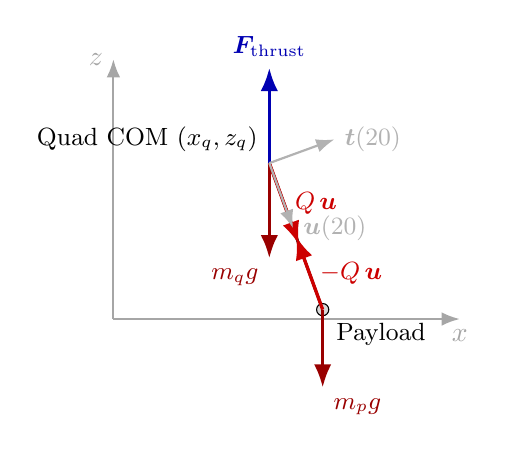
\begin{tikzpicture}[scale=1.1,
        force/.style={-Latex,very thick},
        axis/.style={-Latex,thick,gray!70},
        rope/.style={line width=1pt},
        note/.style={font=\small}
    ]
    
    % --- World axes ---
    \draw[axis] (0,0) -- (4,0) node[below] {$x$};
    \draw[axis] (0,0) -- (0,3) node[left] {$z$};
    
    % --- Quad position and geometry ---
    \coordinate (Q) at (1.8,1.8);
    \def\phi{20}
    \def\L{1.8}
    \def\theta{15}
    \coordinate (u) at ({sin(\phi)},{-cos(\phi)});
    \coordinate (t) at ({cos(\phi)},{sin(\phi)});
    \coordinate (P) at ($(Q)+\L*(u)$);
    
    % --- Rope and payload ---
    \draw[rope] (Q) -- (P);
    \filldraw[fill=gray!30,draw=black] (P) circle (2pt) node[below right=2pt, note] {Payload};
    
    % --- Forces on quad ---
    \draw[force,blue!70!black] (Q) -- ++(0,1.1) node[above, note] {$\bm{F}_{\text{thrust}}$};
    \draw[force,red!80!black] (Q) -- ($(Q)+1.0*(u)$) node[midway, right, note] {$Q\,\bm{u}$};
    \draw[force,red!60!black] (Q) -- ++(0,-1.1) node[below left, note] {$m_q g$};
    \node[note] at (Q) [above left=1pt] {Quad COM $(x_q,z_q)$};
    
    % --- Forces on payload ---
    \draw[force,red!80!black] (P) -- ($(P)+-0.9*(u)$) node[midway, right, note] {$-Q\,\bm{u}$};
    \draw[force,red!60!black] (P) -- ++(0,-0.9) node[below right, note] {$m_p g$};
    
    % --- Unit vectors ---
    \draw[-Latex,thick,gray!60] (Q) -- ($(Q)+0.8*(u)$) node[right, note] {$\bm{u}(\phi)$};
    \draw[-Latex,thick,gray!60] (Q) -- ($(Q)+0.8*(t)$) node[right, note] {$\bm{t}(\phi)$};
    
    \end{tikzpicture}
    \caption{Free-body diagram showing the forces acting on the quadcopter and the tethered payload.}
    \label{fig:fbd}
\end{figure}

\subsection{Tether Geometry and Kinematic Derivations}
\label{ap:tether_derivation}

We consider planar motion of a quadcopter with a payload suspended beneath it by a massless, inextensible tether of variable length $\ell$. The tether configuration is parameterised by the swing angle $\phi$, measured from the vertical. Unit vectors aligned with and perpendicular to the tether are defined as
\[
\bm{u}(\phi) =
\begin{bmatrix}
\sin\phi \\[2pt] -\cos\phi
\end{bmatrix},
\qquad
\bm{t}(\phi) =
\begin{bmatrix}
\cos\phi \\[2pt] \sin\phi
\end{bmatrix}.
\]

The payload position is expressed as
\[
\bm{p}_p =
\begin{bmatrix}
x_q \\ z_q
\end{bmatrix}
+ \ell\,\bm{u}(\phi),
\]
and differentiation yields
\[
\ddot{\bm{p}}_p =
\begin{bmatrix}
\ddot{x}_q \\[2pt] \ddot{z}_q
\end{bmatrix}
+ (\ddot{\ell} - \ell \dot{\phi}^{2})\, \bm{u}
+ (2\dot{\ell}\dot{\phi} + \ell \ddot{\phi})\, \bm{t}.
\]

These expressions are used to derive the payload swing and tether tension equations presented in the main text.

\subsection{PID Controller Implementation Details}
\label{ap:pid}

\subsubsection{Cascaded Control Structure}

The PID controllers are arranged in a cascaded architecture, as shown in Fig.~\ref{fig:cascade}. Outer-loop controllers generate reference commands for inner-loop controllers, which stabilise the quadcopter attitude and vertical motion.

\begin{figure}[t]
    \centering
    \includegraphics[width=\linewidth]{figs/PID.png}
    \caption{Cascaded PID controller diagram}
    \label{fig:cascade}
\end{figure}

\subsubsection{Control Allocation}

The translational and rotational control outputs are mapped to individual rotor thrusts using a standard mixing matrix:
\[
\begin{bmatrix}
T_1 \\ T_2 \\ T_3 \\ T_4
\end{bmatrix}
= M
\begin{bmatrix}
u_z \\ u_\theta
\end{bmatrix},
\]
where $M$ is determined by the quadcopter geometry and rotor configuration.

\subsubsection{Anti-Windup and Saturation Handling}

To ensure stable behaviour under actuator limits, saturation bounds are imposed on all control outputs. Integral windup is mitigated by freezing the integral term whenever saturation occurs in a direction that would further increase the error:
\[
\text{if } (u_i > u_{\max} \land e_i > 0) \;\text{or}\; (u_i < u_{\min} \land e_i < 0), \quad \dot{I}_i = 0.
\]
This prevents integrator accumulation during saturation and enables smooth recovery once the system re-enters the linear operating regime.

\section{\vehicle\ Specification of Formal Properties}
\label{app:vehicle-spec}

This appendix provides the complete \vehicle\ specification of the formal properties
evaluated in Section~\ref{sec:vehicle-properties}. We
encode (i) the bounded input domain, (ii) the neural controller with the same
normalisation pipeline used at training time, and (iii) Properties~P1--P3 as universally
quantified formulas over the bounded input space. 




\section{Additional Explainability Visualizations}
\label{app:xai}

This appendix provides supplementary LIME and Integrated Gradients (IG) visualisations referenced in the main text (Section~\ref{sec:adv_xai}). We include per-sample LIME heatmaps for the normally trained and adversarially trained controllers, as well as per-sample difference maps that highlight how local feature reliance changes after adversarial training. We also report representative IG bar plots (clean vs.\ adversarial) together with the corresponding LIME drift values to illustrate stability under attack.

\begin{figure}[t]
    \centering
    \includegraphics[width=\linewidth]{figs/xai/lime_normal_per_sample.png}
    \caption{\textbf{Normal model: LIME feature importance per sample.} Each panel shows a heatmap of absolute LIME weights (\#outputs $\times$ \#features) for a randomly selected test sample. Darker cells indicate stronger local reliance.}
    \label{fig:lime_normal_per_sample}
\end{figure}

\begin{figure}[t]
    \centering
    \includegraphics[width=\linewidth]{figs/xai/lime_advtrained_per_sample.png}
    \caption{\textbf{Adversarially trained model: LIME feature importance per sample.} Compared to the normal model, feature importance is generally less spiky, suggesting reduced reliance on brittle feature pathways.}
    \label{fig:lime_adv_per_sample}
\end{figure}

\begin{figure}[t]
    \centering
    \includegraphics[width=\linewidth]{figs/xai/lime_diff_per_sample.png}
    \caption{\textbf{Per-sample change in LIME importance after adversarial training.} Heatmaps show $\Delta w = w_{\text{adv-trained}} - w_{\text{normal}}$ (per output $\times$ feature). Blue indicates decreased reliance after adversarial training; red indicates increased reliance.}
    \label{fig:lime_diff_per_sample}
\end{figure}


\begin{figure}[t]
    \centering
    \includegraphics[width=0.92\linewidth]{figs/xai/ig_clean_vs_adv_normal.png}
    \caption{\textbf{Normal model: Integrated Gradients (clean vs.\ adversarial) with LIME drift.} The paired bars show IG attributions per feature for output $j{=}0$ on the clean input $x$ and the adversarial input $x_{\mathrm{adv}}$. The reported LIME drift ($0.565$) indicates a larger change in local explanation under attack.}
    \label{fig:ig_lime_normal}
\end{figure}

\begin{figure}[t]
    \centering
    \includegraphics[width=0.92\linewidth]{figs/xai/ig_clean_vs_adv_advtrained.png}
    \caption{\textbf{Adversarially trained model: Integrated Gradients (clean vs.\ adversarial) with LIME drift.} Compared to the normal model, both the IG profile shift and the LIME drift are smaller ($0.228$), indicating more stable feature reliance under adversarial perturbations.}
    \label{fig:ig_lime_advtrained}
\end{figure}

\end{document}